\documentclass[../main.tex]{subfiles}

%TODO ändern der PHP File Namen, da sie nun hier mit einem sauberen Namen vorausgestetzt werden

\begin{document}
	\chapter{Die Server}
	Im folgenden Kapitel wird auf die beiden Server eingegangen, welche für die Studnetz Applikation verwendet werden. Zuerst werden die mitwirkenden Komponente jeweils einzeln erläutert. Die eigentliche Implementation folgt dann in Kapitel \ref{implementationServer}. Ein schematischer Überblick des Verhältnisses der beiden Server zum Client findet sich in Abbildung \ref{ServerClientSchema}.
	
	\begin{figure} 
		\centering
		\includegraphics[width=\textwidth, height=0.95\textheight]{./images/Scheme.pdf}
		\caption{Schematische Übersicht über die beiden Server und deren Beziehung zum Client (Quelle: Eigene Darstellung)}
		\label{ServerClientSchema}
	\end{figure}
	
	\section{Webserver}
	Bei den beiden in der Applikation verwendeten Server handelt es sich genau genommen um sogenannte Webserver. Ein Webserver beschreibt eine Software, welche das Abrufen von lokalen Diensten (z.B. Programme oder Skripte) und gespeicherten Daten über das Internet ermöglicht. Clients sind dann in der Lage, über die IP-Adresse des Webservers die bereitgestellten Dienste und Daten aufzurufen. Der Webserver ist ebenfalls in der Lage, Antworten auf Anfragen der Clients zurückzusenden. 
		
 	Skripte, die auf dem Server ausgeführt werden ermöglichen den Zugriff auf eine sich ebenfalls auf dem Server befindende Datenbank. Dafür beliebte Skriptsprachen sind Sprachen wie PHP (siehe Kapitel \ref{php}), Ruby, Python oder Pearl. Diese Skripte sind in der Lage, Anfragen an die Datenbank zu stellen und Antworten zu formulieren, welche dann vom Webserver an den Client zurückgeschickt werden können. Eine direkte Kommunikation zwischen Datenbank und Client findet auf einem Webserver so gut wie nie statt.
	
	\subsection{Apache Server}
	Der \emph{Apache HTTP Server} ist eine Webserver Software. Sie wurde 1995 von der \emph{Apache Group} veröffentlicht und besitzt sich seit 1999 in Besitz der \emph{Apache Software Foundation}. Apache HTTP Server darf kostenlos verwendet werden und ist heute der meist verwendete Webserver weltweit. \cite{apache}
	
	\subsection{PHP}\label{php}
	PHP ist eine Open-Source Skriptsprache, welche grosse Beliebtheit in der serverseitigen Webentwicklung findet. Die Abkürzung PHP ist ein rekursives Akronym für \emph{Hyptertext Preprocessor} und wurde speziell für die Webprogrammierung entwickelt. Sich auf Webservern befindende PHP Skripte bieten den grossen Vorteil, dass sie jeweils nur auf dem Server ausgeführt werden. Somit ist es Clients zwar möglich die Skripte via Webadresse auf einem Webserver auszuführen, bekommen jedoch die Codestruktur des PHP Skriptes nie zu Gesicht. \cite{PHP} Im Skript selber wird eine Antwort formuliert, welche dann vom Webserver an den Client zurückgeschickt werden kann. Die Form der Antwort unterscheidet sich dabei stark von Anwendung zu Anwendung. Antworten können in Sprachen wie HTML, JSON oder JavaScript verfasst sein, wobei jedoch auch Bild- und PDF-Dateien durchaus als Antwortformate in Frage kommen. \cite{PHP:function}
	
	\subsection{JSON}
	JSON ist eine Abkürzung für \emph{JavaScript Object Notation} und ist eine Datenformat, welches für den Austausch von strukturierten Daten entwickelt wurde. Bei der Entwicklung wurde dabei besonders auf drei Kriterien geachtet: Lesbarkeit für Menschen sowie einfaches Generieren sowie Parsen auf Seiten des Computers. Diese sehr gut umgesetzten Eigenschaften und seine Plattformunabhängigkeit  machen JSON zu einem äusserst effizienten Datenaustauschformat für einfachere Datentypen und wird besonders in der Webentwicklung gerne verwendet. \cite{JSON}
	
	\section{Datenbanken} \label{Datenbanken}
	Eine der wohl wichtigsten Aufgaben von Computern ist das Speichern, Verwalten und Manipulieren von Informationen. Anwendungen, die sich hauptsächlich mit dieser Aufgabe beschäftigen werden allgemein als \emph{Datenbanken} bezeichnet. Sie haben die Aufgabe, Informationen systematisch zu ordnen, zu speichern und bei Bedarf zu verändern. Grundsätzlich bezeichnet der Begriff Datenbank gleich zwei Dinge auf einmal. Zum einen wird ein strukturierter Speicher von Informationen als Datenbank bezeichnet und zum anderen auch die Anwendung, die das Verwalten der Daten überhaupt erst ermöglicht. Solche Anwendungen werden als \emph{Database Management System} (DBMS) bezeichnet und sind meist hochkomplex in ihren Funktionsweisen, um die effiziente Verwaltung von selbst riesigen Datenmengen zu ermöglichen. \cite{IT-Handbuch} Datenbanken kommen oftmals auf zentralen Servern zum Einsatz, wo zum Beispiel die Benutzer eines Webdienstes oder die Bestellungen einer Firma aufgelistet werden. Sie stellen den dynamischen Speicher eines Servers bzw. Webservers dar.
	
	\subsubsection*{Tabellenstrukturen}
	Die Informationen in einer Datenbank werden meist in einer auf Tabellen basierenden Struktur gespeichert. Dabei wird eine einzelne Zeile in der Tabelle als Datensatz oder Eintrag bezeichnet, während die verschiedenen Spalten Felder genannt werden. Beim Erstellen einer solchen Tabelle werden zuerst die verschiedenen Felder bestimmt. Ihnen wird ein Name gegeben, der beschreibt, was darin gespeichert werden soll. Hinzu kommt ein Datentyp, der angibt um was es sich bei diesem Feld handelt (z.B. eine Zahl oder einen kurzen Text). Es ist ebenfalls möglich einem Feld einen \emph{Default}-Wert zuzuschreiben. Dieser wird dann für einen Datensatz verwendet, wenn der Wert des Feldes sonst nicht definiert wurde. Zuletzt ist es noch möglich, einem Feld speziellere Eigenschaften zuzuschreiben. Dazu gehört unter anderem eine Funktion mit dem Namen \emph{auto\_increment}. Sie bewirkt, dass diesem Feld bei einem neu eingetragenen Datensatz automatisch ein in der Tabelle einzigartiger Wert des Typen Integer (Datentyp für natürliche Zahlen) zugewiesen wird.
	
	Es ist dabei anzumerken, dass verschiedene Datenbanken oft verschiedene, variierende Datenstrukturen verwenden. Die soeben beschriebene Tabellenstruktur trifft hauptsächlich auf die beiden verbreiteten SQL Datenbanken MySQL und MariaDB zu. Dies schliesst jedoch keineswegs andere Strukturen aus, wie solche, die später in Kapitel \ref{firebaseRealtime} thematisiert werden werden.
	
	\subsubsection*{Datenbanktypen}
	Datenbanken selber können in verschiedene Typen eingeteilt werden, die alle ihre eigenen Vor- und Nachteile mit sich bringen. Die einfachste Form eines Datenbanktyps ist wohl die \emph{Einzeltabellendatenbank}. Sie besteht aus nur einer Tabelle, in welcher alle Informationen abgespeichert werden. Sie eignet sich gut für kleine, übersichtliche Tabellenstrukturen wie zum Beispiel eine einfache Liste von Adressen. Die Einzeltabellendatenbank stösst jedoch spätestens dann an ihrer Grenzen, wenn die Informationen nicht mehr in nur einer, sondern gleich mehreren Tabellen gespeichert werden sollen. Hier tritt ein anderer Datenbanktyp ins Spiel. Eine \emph{relationale Datenbank} ist in der Lage, verschiedene Tabellen logisch miteinander zu verknüpfen und sich darin zu orientieren. Diese logische Verknüpfung ist möglich aufgrund eindeutiger Eigenschaften eines Datensatzes. Dies kann zum Beispiel eine Kundennummer oder ein Name sein. Ein solches Feld wird auch als \emph{Key} bezeichnet. Wichtig dabei ist, dass jeder Key nur einmal in einer Tabelle vorkommt, da ansonsten keine eindeutige Verknüpfungen möglich sind. Die Anwendung zur Verwaltung einer solchen relationalen Datenbank wird \emph{Relational Database Management System} (RDBMS) genannt. \cite[S. 745 - 751]{IT-Handbuch}
	
	\subsection{Die MySQL Datenbank}
	Eines der am weitesten verbreiteten RDBMS ist die MySQL Datenbank. Das System wurde ursprünglich von den drei Gründern Allan Larsson, Michael Widenius und David Axmark 1995 entwickelt, wurde später von \emph{Sun Microsytems} aufgekauft und gelangte schlussendlich in den Besitz des amerikanischen Softwareherstellers \emph{Oracle}. MySQL ist unter einem dualen Lizenzsystem eingetragen, sodass die Software zum einen unter eine \emph{General Public Licence} (GPL) \cite{GPL}, aber auch unter eine proprietäre Lizenz \cite{proprietaereLizenz} gestellt ist. \cite{tecmint.com} Das MySQL System darf aufgrund der GPL gratis heruntergeladen, installiert und modifiziert werden.
	
	MySQL Datenbanken sind besonders bei der Betreibung von Webdiensten aller Art von grosser Beliebtheit. Sie befinden sich dann, wie bereits in Kapitel \ref{Datenbanken} erwähnt, auf einem zentralen Server. Mithilfe sogenannter \emph{Queries} (Datenbank Abfragen) ist es dem Server möglich mit der Datenbank zu interagieren. Solche Queries sind im Falle einer MySQL Datenbank in der Datenbanksprache \emph{SQL} (Structured Query Language) formuliert. Queries können in vier Arten von Abfragen unterteilt werden: \cite[S. 760]{IT-Handbuch}
	
	\begin{itemize}
		\item Auswahlabfragen (\emph{Select Queries}) geben den Inhalt von einem oder mehreren Feldern aus einer oder verschiedenen Tabellen zurück. Dabei kann bei Bedarf nach Kriterien gefiltert werden, um die Suche nach bestimmten Datensätzen einzugrenzen.\cite[S. 746]{IT-Handbuch}
		\item Einfügeabfragen (\emph{Insert Queries}) fügen einen neuen Datensatz zu einer bestehenden Tabelle hinzu. \cite[S. 746]{IT-Handbuch}
		\item Änderungsabfragen (\emph{Update Queries}) ändern bestimmte oder alle Felder eines bestehenden Datensatzes in einer Tabelle. \cite[S. 746]{IT-Handbuch}
		\item Löschabfragen (\emph{Delete Queries}) löschen einen Datensatz aus einer Tabelle. \cite[S. 746]{IT-Handbuch}
	\end{itemize}
	
	\subsection{Firebase} \label{DieFirebaseDatenbank}
	Firebase ist eine  Entwicklungsplattform für Webapplikationen, welche seit 2014 von Google angeboten wird. Firebase entwickelte sich aus dem 2011 gegründete Startup \emph{Envolve} der beiden Gründern James Tamplin und Andrew Lee. Das Ziel von Envolve war es, Kunden eine API (\emph{Application Programming Interface}) zu bieten, mit welcher in Echtzeit synchronisierte Chatfunktionen einfach realisiert werden können. Nachdem jedoch viele Benutzer die API für andere Anwendungen als Chats verwendeten, ja sogar einzelne Spielentwickler sie für eine Synchronisation verschiedener Clients in Echtzeit verwendeten, begann die Entwicklung sich auf das Anbieten einer API für Echtzeitsysteme zu konzentrieren. Der Erfolg war gross und 2014 wurde das Unternehmen von Google aufgekauft. Google entwickelte aus Envolve daraufhin eine Plattform, welche verschiedenste Tools zur Webdienstentwicklung beinhaltet und heute unter dem Namen Firebase vermarktet wird. Firebase bietet sowohl Tools für die Entwicklung neuer Dienste wie Echtzeitdatenbanken, Authentifizierungsfunktionen und Crashanalysen, aber auch für das Unterhalten von bestehenden Diensten. Beispiele für ein solche Tools zur Unterhaltung bestehender Dienste wären zum Beispiel das Senden von Push-Benachrichtigungen an alle Clients oder das Überwachen von geschalteter Werbung innerhalb der Clients. Die Tools dürfen in einem begrenzten Rahmen gratis verwendet werden und sind daher sehr attraktiv für kleinere Entwicklerunternehmen und Lernende, eignen sich aber durchaus auch für grössere Unternehmen. \cite{Firebase}
	
	\subsubsection{Die Firebase Echtzeitdatenbank} \label{firebaseRealtime}
	Wie bereits erwähnt, bietet Firebase unter anderem eine sogenannte Echtzeitdatenbank (Realtime Database) an. Diese Echtzeitdatenbank ist eine NoSQL Datenbank und unterscheidet sich in ihrer Funktionsweise stark von traditionellen Datenbanken wie MySQL oder MariaDB. Anders als traditionelle Datenbanken auf Webservern agieren Echtzeitdatenbanken nicht nur passiv auf Anfragen, sondern teilen den Clients aktiv mit, wenn sich ein Datensatz verändert hat (Push-Based Data Access) und halten sie so immer auf dem neusten Stand. Solche Mitteilungen über Datensatzänderungen bezeichnet mal allgemein als \emph{Pushes}. Echtzeitdatenbanken werden besonders dann eingesetzt, wenn sich ein Datensatz häufig oder jederzeit ändern kann und es notwendig ist, dass die Clients ohne grosse Verzögerung davon unterrichtet werden. \cite{RealtimeDatabase} Bei der Firebase Echtzeitdatenbank ist es nicht einmal nötig, dass die Clients zur Zeit des Pushes online sind. Sie werden beim nächsten Start automatisch dann mit dem Datensatz auf der Datenbank abgeglichen und aktualisiert. Ein weiterer grosser Unterschied der Firebase Echtzeitdatenbank zu einer MySQL Datenbank ist, dass Daten nicht mehr in Tabellenstruktur gespeichert werden. Vielmehr wird ein System verwendet, welches optisch an ein Verzeichnissystem erinnert, wobei es sich jedoch nicht wirklich um Verzeichnisse handelt. Genauer genommen werden die Daten als JSON-Objekte gespeichert und strukturiert. Dabei ist es möglich, mehrere JSON-Objekte jeweils ineinander abzuspeichern, was zu dieser Verzeichnis artigen Struktur führt. Eine solche Struktur nennt man dann auch einen \emph{JSON-Tree}, wobei die einzelnen Elemente als \emph{Nodes} (Knoten) bezeichnet werden. Diese Eigenschaft macht die Firebase Echtzeitdatenbank zu einer äusserst flexiblen Datenbank, da sie dadurch kaum an vorgegebene Strukturen wie Tabellen oder Felder gebunden ist. \cite{firebaseStructure}\cite{FirebaseRTDB}
	
	
	\section{Sicherheit der Passwörter in einer Datenbank}
	Generell gilt, dass Passwörter nie in ihrer reinen Form irgendwo gespeichert werden dürfen, sofern sie vor potentiell bösartigen Angriffen geschützt sein sollen. Um eine Lesbarkeit der Passwörter zu vermeiden wird oft ein sogenannter Prozess des Hashens und des Salzens der Passwörter angewandt. 
	
	\subsection{Hashen}
	Hashen ist ein mathematisches Verfahren, das im Grunde genommen die Bits einer Eingabe vermischt und zu einem Ergebnis bringt, welches nicht mehr in seine Ursprungsform zurückgerechnet werden kann. Der grosse Vorteil dabei ist, dass jede Eingabe einen absolut einzigartigen Hash bekommt. Es kann keine Kollisionen geben, ausser die Eingabe ist gleich, jedoch dazu etwas später mehr. Weiter sind alle Hashes unabhängig von der Länge der Eingabe immer gleich lang. Es kann also nicht einmal die Passwortlänge aus einem Hash herausgelesen werden. Das Hashen der Passwörter wäre also eine schon deutlich sicherer Methode, um die Passwörter auf dem Server zu speichern. Somit würde beim Login jeweils das vom Benutzer/der Benutzerin eingegeben Passwort ebenfalls gehasht werden und anschliessend mit dem auf dem Datenbank gespeicherten Hash verglichen werden. Da es keine Kollisionen geben kann, wäre dies eine durchaus sichere Variante, um die Passwörter für einen Menschen unleserlich zu machen. 
	
	Doch leider reicht dies noch nicht. Hashes sind mittlerweile gut dokumentiert und ein gehashtes Wort kann einfach in einer Suchmaschine eingegeben werden und mit etwas Glück wird einem bereits in den ersten Ergebnissen das gehashte Wort in Klartext angezeigt. Zudem kommt die Gefahr, dass zwei Benutzer in einer Datenbank zufällig das gleiche Passwort verwenden könnten. Dann wäre ihr gehashtes Passwort ebenfalls identisch. Solche Gegebenheiten können von einem potenziellen Angreifer ausgenutzt werden. \cite{defuse} \cite{security}
	
	\subsection{Salzen}
	Um dieser Problematik vorzubeugen wird ein zweiter Prozess, der allgemein als Salzen bezeichnet wird, angewandt. Salzen ist ein Verfahren, bei welchem jeweils vor oder nach der eigentlich zu hashenden Eingabe noch eine Reihe von zufällig generierten Werte angehängt wird. Diese Werte sind dann das \emph{Salz} des Hashes, da sie den Hash komplett verändern, wie ein Gewürz den Geschmack einer Speise verändert. Die Idee ist, dass jeweils jeder Benutzer sein eigenes zufällig generiertes Salz zu seinem Passwort bekommt. Das Salz wird ebenfalls in der Datenbank gespeichert und muss dabei nicht einmal verschlüsselt werden. Es kann direkt neben dem gehashten Passwort gespeichert sein. Somit wird jeweils bevor das Passwort gehasht wird das Salz dem Passwort angehängt. Sofern jeder Benutzer ein eigenes Salz besitzt, kann es zu keinen Überschneidungen bei den Passwörtern kommen. Um die Einzigartigkeit der Salze zu gewährleisten wird daher zu Salzen mit mehr als 16 Bytes Länge geraten. Die Chance für eine Überschneidung fällt dann in einen vernachlässigbaren Bereich. 
	
	Selbst wenn nun ein Angreifer in Besitz sämtlicher Passwörter und Salze der Datenbank käme, wäre es ihm noch immer nicht möglich, die Passwörter der einzelnen Benutzern herauszufinden, ohne dafür auf einen Bruteforce-Attack (Ausprobieren aller möglicher Zeichenkombinationen) für jedes einzelne Passwort zurückzugreifen. Diese Verfahren gilt daher allgemein als sicher. \cite{defuse} \cite{security}
	
	\subsection{bcrypt}
	Innerhalb der Studnetz Applikation wird für diesen Prozess die kryptologische Hashfunktion \emph{bcrypt} verwendet. Bcrypt ist speziell für das sichere Speichern von Passwörtern entwickelt worden und hasht Eingaben automatisch mit einem Salz. Die Besonderheit an bcrypt ist, dass sie im Gegensatz zu anderen populären Hashfunktionen wie die Algorithmen der \emph{SHA}-Familie (Secure Hash Algorithm) nicht auf Effizienz optimiert worden ist. Das Ziel von bcrypt ist es stattdessen, den Aufwand für das Hashen einer Eingabe möglichst aufwändig zu halten. Der Rechenaufwand kann dabei manuell eingestellt werden. Wenn der Rechenaufwand genug hoch ist (gewöhnlich wird dafür der Wert 10 oder 11 verwendet) macht dies Anwendung von Bruteforce-Attacken zu einem äusserst zeitaufwendigen Prozess, die bei einem einigermassen sicheren Passwort kaum von Erfolg gekrönt werden. \cite{bcrypt}
	
	Um dies etwas deutlicher zu machen verweise ich auf einen Benchmarktest von Jeremy M. Gosney, der diverse Hashalgorithmen auf ihre Effizienz verglich. Dabei ist es ihm möglich gewesen, mithilfe der SHA-512 Hashfunktion pro Sekunde ca. 1'075 Millionen Hashes zu generieren, während unter den gleiche Umständen nur ca. 13'100 bcrypt Hashes pro Sekunde mit dem Kostenwert 5 generiert werden konnten. \cite{benchmark}
	
	\section{Implementation in der entwickelten Applikation}\label{implementationServer}
	Der folgende Abschnitt des Kapitels befasst sich mit der eigentlichen Implementation der in diesem Kapitel bereits erläuterten Komponenten in der entwickelten Applikation.
	
	
	\subsection{Die verwendeten Server}
	Innerhalb der Studnetz-Applikation werden zwei verschiedene, unabhängige Server verwendet.
	
	Auf der einen Seite findet sich ein herkömmlicher Apache HTTP Webserver, welcher mir freundlicherweise von Herrn Andreas Umbach zur Verfügung gestellt worden ist und sonst für das Ergänzungsfach Informatik verwendet wird. Auf ihm befindet sich eine MySQL Datenbank und diverse PHP-Dateien. Er wird für das Speichern der Accountdaten von den einzelnen Benutzern/Benutzerinnen verwendet.
	
	Auf der anderen Seite findet sich ein mit einem Google Account verbundener Firebase Server mit einer Echtzeitdatenbank. Er wird für die Chats der Applikation verwendet.
	
	\subsection{Datenbankstrukturen}
	Das geschickte Planen und Strukturieren von Datenbanken ist wohl einer der wichtigsten Schritte für die Entwicklung einer Applikation, die von auf einer Datenbank basiert. Oft ist dies auch einer der ersten Schritte in der Planung einer Applikation überhaupt, da die Datenbankstruktur oft massgebend die Funktion der Clients und der angebotenen Dienste bestimmt. Dabei sollte zuerst jeweils einmal festgelegt werden, welche Aufgaben und Ziele die Datenbank erfüllen soll. Dann müssen, im Falle von tabellenbasierten Datenbanken, Tabellen und ihre Felder so strukturiert werden, dass diese Anforderungen erfüllt werden können. 
	
	Ein Weg, die geplante Struktur zu visualisieren, kann das Erstellen eines \emph{Entity-Relationship-Models} (ERM) sein. ERMs eignen sich gut für das Darstellen der einzelnen Tabellen und ihren Feldern, wie auch das Verhältnis, in welchem die Tabellen zu einander stehen. Hierzu werden die verknüpften Tabellen mit einander verbunden und dabei das verbindende Feld markiert (z.B. eine Kundennummer oder Bestellnummer). Die Verhältnisse werden dann im Schema (1, 1) über die Verbindung geschrieben. Die erste Ziffer gibt dabei die minimale Anzahl an herrschenden Beziehungen an, die zweite Ziffer die maximale Anzahl. Im Falle von (1, 1) Beziehungen bedeutet dies, dass es immer genau eine solche Beziehung geben darf und auch muss. Sind die Anzahl Beziehungen unlimitiert, stehen anstelle der Ziffern stellvertretend die Variablen \emph{m} und \emph{n}. Das für die MySQL Datenbank dieser Arbeit verwendete ERM ist in Abbildung \ref{ERM} dargestellt.
	
	\begin{figure} 
		\centering
		\makebox[\textwidth][c]{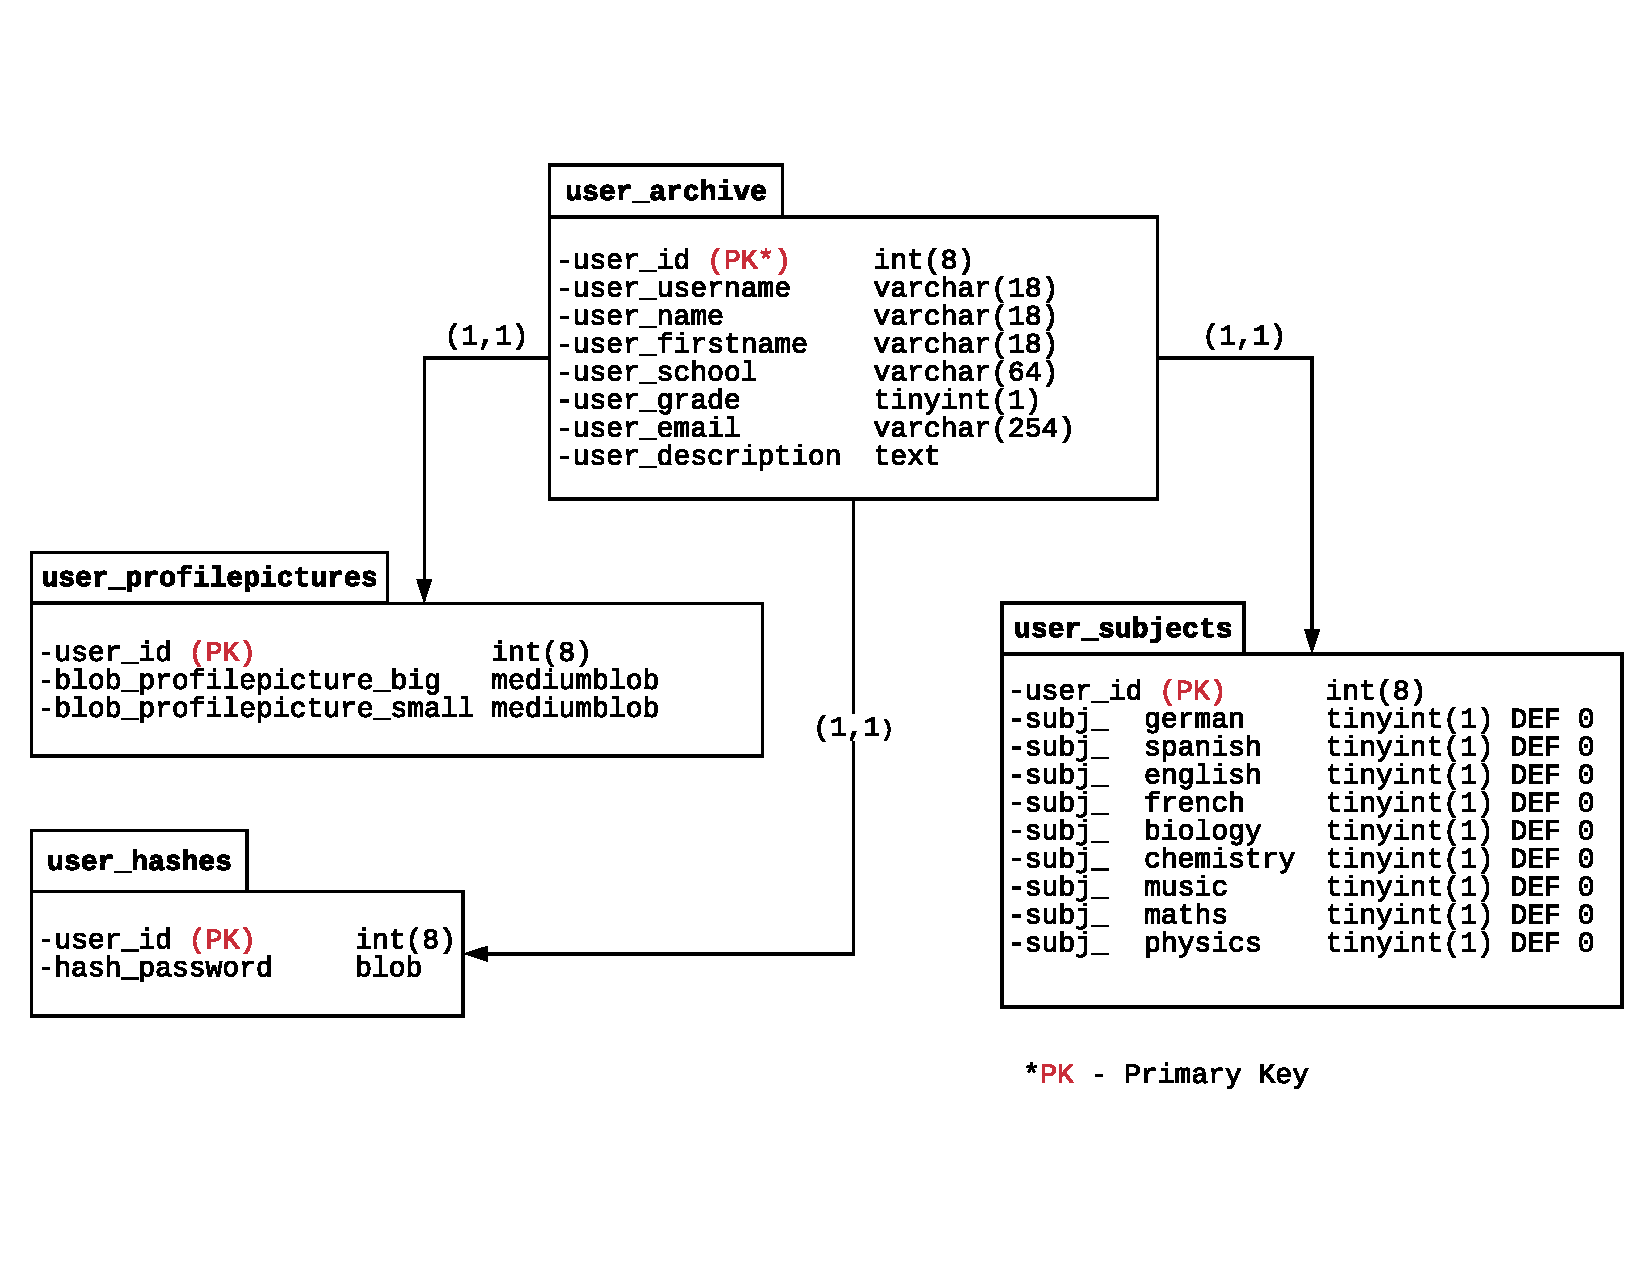
\includegraphics[width=1.2\textwidth]{./images/ERM.pdf}}
		\caption{Das ERM der MySQL Datenbank (Quelle: Eigene Darstellung)}
		\label{ERM}
	\end{figure}
	
	\subsubsection{MySQL Datenbankstruktur} \label{MySQLStructure}
	Die MySQL Datenbank der entwickelten Applikation umfasst vier Tabellen:
	
	\begin{itemize}
		\item Die \emph{user\_archive} Tabelle beinhaltet allgemeine Informationen zu registrierten Benutzern/Benutzerinnen. Dazu gehören Informationen wie Benutzername, Vor- und Nachname, Email, Schule, Klasse und Beschreibung. Zudem kommt noch eine Benutzer ID (\emph{user\_id}), welche jedem Benutzer automatisch über die auto\_increment Funktion beim Registrieren zugewiesen wird und für jeden Benutzer einzigartig ist.
		\item Die \emph{user\_profilepictures} Tabelle besitzt drei Felder. Eines für die user\_id, und zwei Felder vom Datentyp \emph{Medium BLOB}, in welchen jeweils eine kleine und eine grosse Variante des Profilbildes eines Benutzers/einer Benutzerin gespeichert wird. Die Bildformate sind dabei jeweils in Forme einer \emph{Base64} kodierten Zeichenkette. Die Base64 Kodierung ermöglicht den sicheren Transfer von Bilddateien vom Client zum Server, ohne dass es dabei zu Datenverlust oder Modifikationen aufgrund von Inkompatibilitäten kommt \cite{base64}. Das Speichern von grösseren Bilddateien in relationalen Datenbanken ist umstritten, da es die Effizienz der Datenbank negativ beeinflussen kann. Man findet hier verschiedene Ansichten. Im Rahmen dieser Arbeit jedoch sollte diese Datenbankkonfiguration keine grösseren Probleme mit sich bringen, weshalb es dabei belassen wurde.
		\item Die \emph{user\_hashes} Tabelle besitzt zwei Felder. Eines für die user\_id und eines für den Hash des Passworts.
		\item Die \emph{user\_subjects} Tabelle beinhaltet Felder für alle von der entwickelten Applikation unterstützten Fächer.
		Mithilfe der Werte 1 und 0 wird angegeben, in welchen Fächern ein Benutzer/eine Benutzerin Nachhilfeunterricht anbietet (1 steht für "Ja", 0 für "Nein").
	\end{itemize}
	
	 Die Hauptaufgabe der vier Tabellen ist das Speichern aller statischen Informationen über die verschiedenen registrierten Benutzer/Benutzerinnen. Die einzelnen Tabellen können alle über die user\_id eines Benutzers miteinander verknüpft werden. Die user\_id ist zudem in allen Tabellen als ihr jeweiliger \emph{Primary Key} markiert. Für die Datenbank bedeutet dies, dass dieses Feld jeweils für jeden Datensatz einen einzigartigen Wert besitzt und für die Unterscheidung der Datensätze optimiert werden soll. Besonders für grosse Datenbanken ist eine geschickte Handhabung solcher Keys von grosser Bedeutung, da sie die Effizienz einer Datenbank drastisch beeinflussen kann.
	
	\subsubsection{Firebase Datenbankstruktur}
	Wie bereits in Kapitel \ref{DieFirebaseDatenbank} erwähnt, ist die Firebase Echtzeitdatenbank etwas anders strukturiert, weshalb das dazu gehörende ERM eine baum-ähnliche Struktur aufweist, wie sie in Abbildung \ref{firebaseTree} dargestellt wird. 
	\begin{figure} 
		\centering
		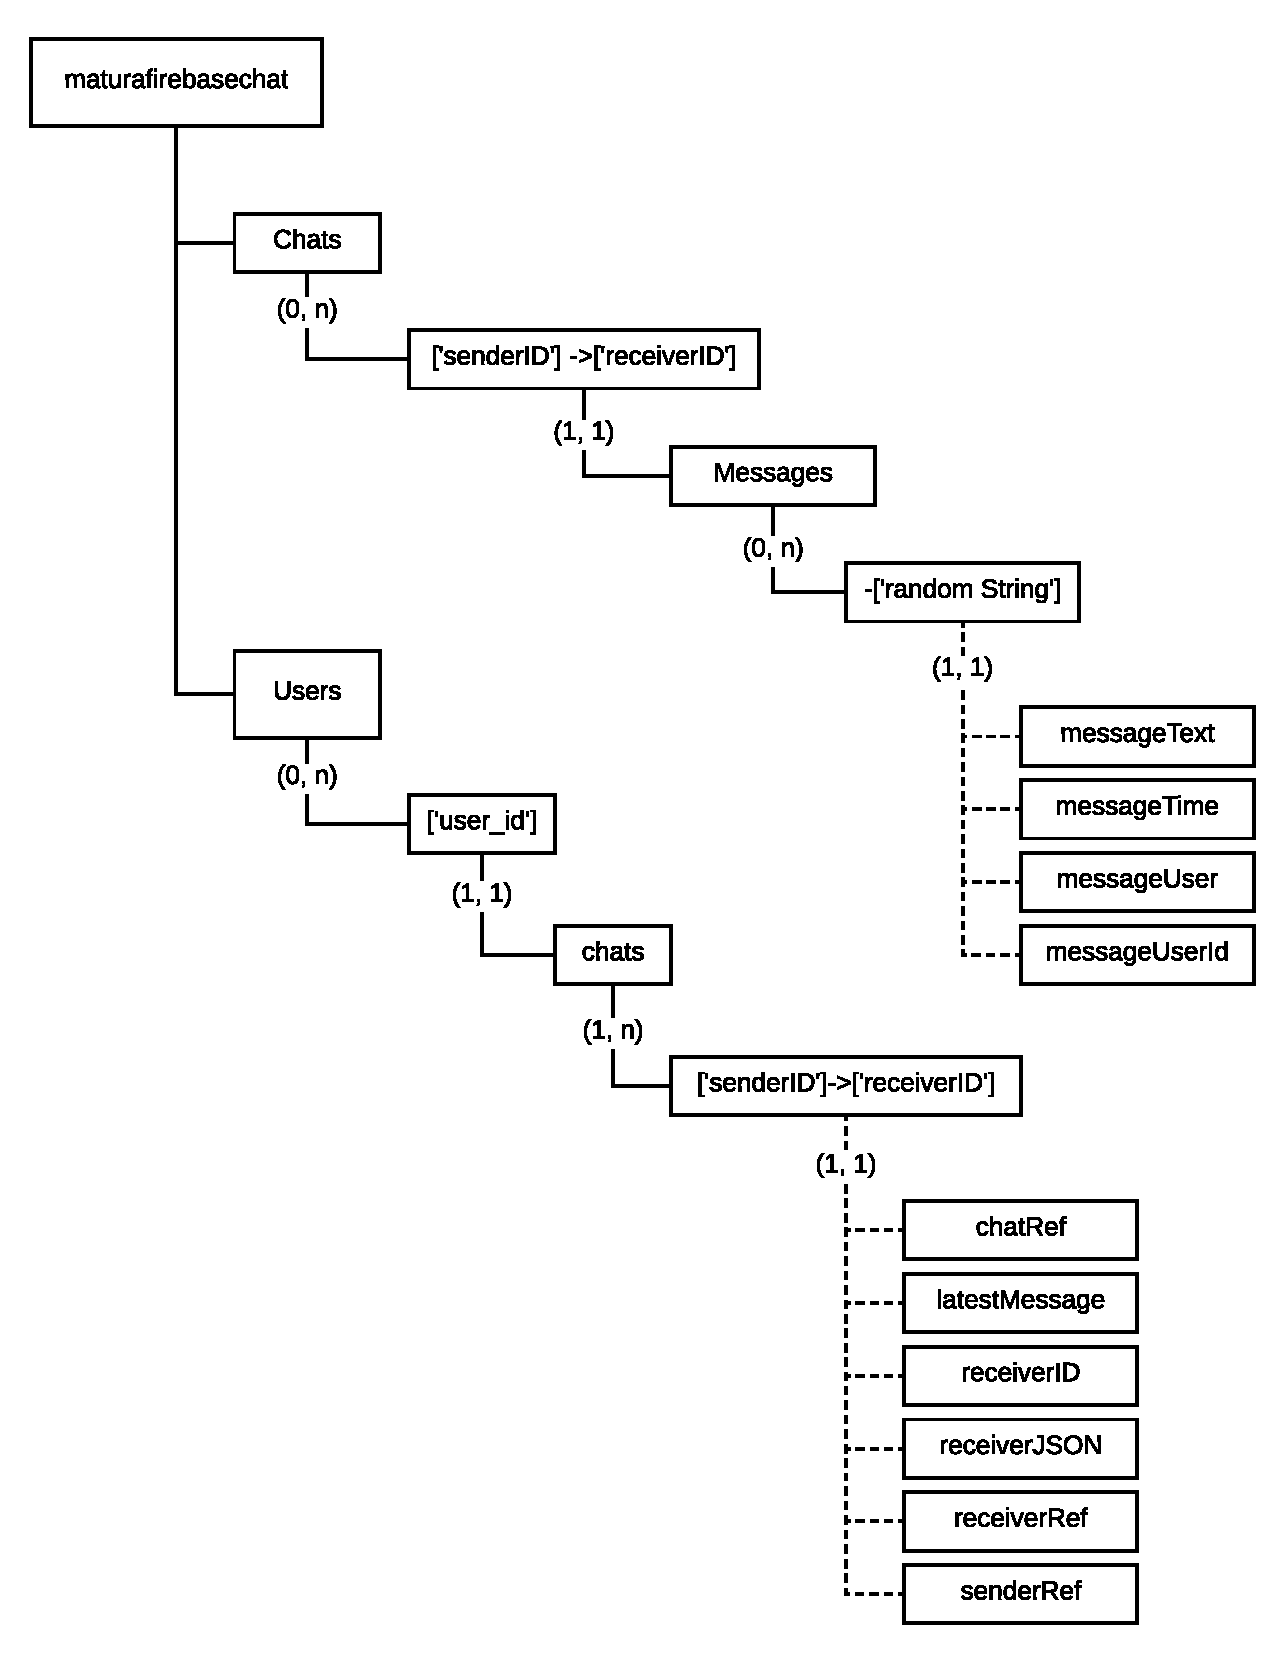
\includegraphics[width=\textwidth]{./images/FirebaseStructure.pdf}
		\caption{Darstellung der Firebase Echtzeitdatenbankstruktur (Quelle: Eigene Darstellung)}
		\label{firebaseTree}
	\end{figure}
	Auf der Abbildung findet sich ein Schema der für die Studnetz Applikation verwendeten Firebase Datenbankstruktur. Dabei kann zwischen den zwei Hauptknoten (Nodes) unterschieden werden. Hierbei ist anzumerken, dass sich die verwendeten Begriffe \emph{Sender} und \emph{Receiver} aus der Sicht des momentan aufgerufenen Profils verwendet werden. Somit sind bei zwei Chatpartnern/Chatpartnerinnen beide aus der einen Sicht der Sender, während sie von der anderen Seite aus der Receiver sind.
	
	\begin{itemize}
		\item Der \emph{Users}-Knoten beinhaltet eine Liste aller Benutzer/Benutzerinnen, die je in einem Chat in der Applikation involviert gewesen sind. Die Knoten für die einzelnen Benutzer/Benutzerinnen wird jeweils mit der user\_id des Benutzers/der Benutzerin aus des MySQL Datenbank gekennzeichnet. Darin findet sich ein Knoten \emph{chats}. Dort werden Knoten für alle Chats aufgeführt, in welchen ein Benutzer/eine Benutzerin involviert ist. Die Knoten sind jeweils so benannt, dass beide user\_ids der am Chat Benutzer/Benutzerinnen herausgelesen werden können. Der Knoten eines Chats enthält die acht für einen Chat relevanten Werte: die Referenz zum Chat, wo die Nachrichten des Chats aufgeführt sind, ein Wert für die zuletzt gesendete Nachricht, die Zeit, zu welcher sie gesendet wurde, der Status, ob sie gelesen wurde,  die Referenzen zu den beiden Benutzern/Benutzerinnen (Sender sowie Receiver), ein JSON-String, in welchem die Benutzerinformationen des Receivers gespeichert sind, und die user\_id des Receivers.
		\item  Der \emph{Chats}-Knoten beinhaltet Knoten für alle Chats, die in der Applikation geöffnet sind. Darin findet sich ein Knoten mit dem Namen \emph{Messages}. Unter diesem Knoten findet man Knoten für alle im Chat gesendeten Nachrichten. Die Knoten der einzelnen Nachrichten tragen dabei jeweils eine generierte Zeichenkette als Namen. Die Nachrichten selber bestehen aus vier Werten: der Nachricht selber, der Zeit, zu welcher die Nachricht gesendet wurde, dem Benutzernamen des Senders und der user\_id des Senders.
	\end{itemize}

	Es ist an dieser Stelle noch interessant zu erwähnen, weshalb die Firebasestruktur auf den ersten Blick etwas überkompliziert erscheinen mag. Der Grund dafür ist eine spezifische Eigenheit von Echtzeitdatenbanken. Anders als bei relationalen Datenbanken ist es in Echtzeitdatenbanken nur schwer möglich, nach Einträgen zu suchen, bei welchen nicht der gesamte Namen bekannt ist. Somit ist es nicht möglich für die Darstellung der Chats auf der Hauptseite einfach nach Einträgen im Chats Ordner zu suchen, in welchen die user\_id des Benutzers/der Benutzerin vorkommt. Deshalb musste eine Alternative gefunden werden, welche sich nun in der Form des User Ordners ausdrückt. Dort werden alle Pfade zu den Chats gespeichert, in welchen ein Benutzer/eine Benutzerin vorkommt. Die Pfade werden beim Eröffnen eines neuen Chats dort eingetragen. Auf diese Weise ist es trotzdem möglich, alle offenen Chats eines Benutzers/einer Benutzerin zu finden, ohne dass eine Suchfunktion benötigt wird.
	
	%\subsection{Hashen und Salzen der Passwörter}
	
	\subsection{PHP Skripte}
	Im folgenden Abschnitt wird nun auf die PHP Skripte eingegangen, die auf dem Webservers der MySQL Datenbank verwendet werden. An dieser Stelle ist anzumerken, dass im folgenden Kapitel für das Hashing des Passwortes von einer PHP Version $\ge 5.3.7$ ausgegangen wird. Da auf dem Ergänzungsfachserver die PHP Version 5.3.29 installiert ist, unterscheiden sich die Namen der Hashfunktionen in der entwickelten Applikation von den in diesem Kapitel beschriebenen Hashfunktionen leicht, die Funktionsweise ist jedoch vergleichbar. Für das Hashing in der entwickelten Applikation  musste wegen der PHP Version eine zusätzliche Bibliothek installiert werden (PHP-PasswordLib by Anthony Ferrera \cite{PWLib}).
	
	Wichtig zu wissen ist jedoch, dass die mit der Bibliothek generierten Hashes bekannterweise Fehler bei der Verwendung von bestimmten \emph{non-ASCII} (American Standard Code for Information Interchange) Zeichen aufweisen können und daher als veraltet gelten. Ein Update wäre also vor einer möglichen Veröffentlichung nötig. \cite{bcryptBug}
	
	\subsubsection{Login}
	Damit ein Client Zugriff auf einen Datensatz eines Benutzers/einer Benutzerin in der Datenbank bekommt, muss sich der Benutzer/die Benutzerin zuerst unter einem bestehenden Account einloggen. Hierzu muss im Client sowohl der Benutzername wie auch das Passwort eines registrierten Accounts eingegeben werden. Danach erfolgt der restliche Login-Prozess auf dem Server.
	 
	Hierzu wird vom Client die \emph{login\_bcrypt.php}-Datei auf dem Webserver via Webadresse aufgerufen. Dabei werden über die \emph{POST}-Methode der eingegebene Benutzername und das Passwort mitgegeben. Diese Werte können innerhalb der PHP-Skriptes verwendet werden. Auf dem Webserver wird überprüft, ob ein Datensatz in der Datenbank existiert, dessen Benutzername dem eingegebene Benutzernamen entspricht. Dies wird über ein sogenanntes \emph{MySQL Statement} getan. Solche Statements sind in der Lage, Anfragen an die verbundene Datenbank zu stellen. In diesem Falle wäre das nun eine Auswahlabfrage (Select Query), die in der user\_archive Tabelle nach einem Datensatz mit dem eingegebenen Benutzername sucht, wobei die Tabelle über einen \emph{INNER JOIN} mit der user\_hashes Tabelle verknüpft wird (siehe Abbildung \ref{SQL:SALT}). Die Fragezeichen stehen stellvertretend für die einzufügenden Werten, die erst später zugewiesen werden. Statements, die auf diese Weise formuliert werden, werden als sogenannte \emph{Prepared Statements} bezeichnet. Sie werden verwendet, um sogenannten \emph{SQL Injektionen} vorzubeugen \cite{preparedstatement}. SQL Injektionen sind bösartige Angriffe auf eine Datenbank, bei welchen anstelle der eigentlich verlangten Eingabe (z.B. einem Benutzernamen oder einem Passwort) SQL Kommandos eingegeben werden, die dann fälschlicherweise von der Datenbank ausgeführt werden \cite{sqlinjection}. 
	
	Bei der Auswahlabfrage in Abbildung \ref{SQL:SALT} darf jeweils nur genau ein Eintrag gefunden werden, da sonst nicht klar wäre, an welchen Account das Login gerichtet ist. Deshalb muss jeder Benutzername in der Datenbank einzigartig sein.
	 %Im ersten Schritt wird vom Client das \emph{salt.php}-File auf dem Server vie Webadresse aufgerufen, wobei dem PHP File mithilfe der POST Methode der eingegebene Benutzername übergeben wird. Dort wird dann anschliessend ein sogenanntes \emph{MySQL Statement} erstellt. Solche Statements sind in der Lage, Anfragen an die verbundene Datenbank zu stellen. In diesem Falle wäre das nun eine Auswahlabfrage (Select Query), die in der user\_archive Tabelle nach einem Datensatz mit dem eingegebenen Benutzername sucht, wobei die Tabelle über einen \emph{INNER JOIN} mit der user\_hashes Tabelle verknüpft wird (siehe Abbildung \ref{SQL:SALT}). Die Fragezeichen stehen stellvertretend für die einzufügenden Werten, die erst später zugewiesen werden. Statements, die auf diese Weise formuliert werden, werden als sogenannte \emph{Prepared Statements} bezeichnet. Sie sind dazu da, um sogenannten \emph{SQL Injektionen} vorzubeugen \cite{preparedstatement}. Bei der Auswahlabfrage in Abbildung \ref{SQL:SALT} darf jeweils nur genau ein Eintrag gefunden werden, da es sonst zu Problemen beim Passwort kommen kann. Deshalb muss jeder Benutzername in der Datenbank einzigartig sein. Wird von der Auswahlabfrage ein Datensatz mit dem eingegebenen Benutzernamen gefunden, wird dem Client das Salz des Benutzers/der Benutzerin in JSON-Format zurückgegeben. 
 
	 \begin{code}
	 	\begin{center}
	 		\begin{minted}[breaklines]{sql}
SELECT user_hashes.hash_password FROM user_archive INNER JOIN user_hashes ON user_archive.user_id = user_hashes.user_id WHERE user_archive.user_username = ?
	 		\end{minted}
	 		\caption{Select Query für das Auslesen des Passwortes eines Benutzers aus der user\_archive Tabelle und der user\_hashes Tabelle (Quelle: Eigene Darstellung)}\label{SQL:SALT}
	 	\end{center}
	 \end{code}
 
 	Wenn ein Ergebnis gefunden werden konnte, wird der Hash des Passwortes aus der Datenbank ausgelesen und mit dem eingegebenen Passwort verglichen. Dies geschieht über die \emph{password\_verify}-Funktion von PHP, welche mit der PHP Version 3.5.7 implementiert wurde (siehe Abbildung \ref{hashcheck}). Wenn das eingegebene Passwort mit dem gehashten Passwort übereinstimmt, wird fortgefahren. 
 	
\begin{code}
 	\begin{center}
 		\begin{minted}[breaklines, mathescape, linenos, tabsize = 5]{php}
<?php
	if(password_verify($user_password, $check['hash_password']) {
		[...] //Auslesen des Datensatzes
	};
?>
 			\end{minted}
 			\caption{Überprüfen eines eingegebenen Passwortes (Quelle: Eigene Darstellung)}\label{hashcheck}
 		\end{center}
 	\end{code}
 	
 	Nun können alle benötigten Informationen über den Benutzer aus der Datenbank über eine Auswahlabfrage ausgelesen werden und im JSON-Format an den Client geschickt werden. Im JSON wird dem Client gleichzeitig mitgeteilt, dass das Login erfolgreich war.
	 
	Sollte jedoch irgendwo in diesem Prozess ein Fehler auftreten, wie zum Beispiel die Verwendung eines nicht existenten Benutzernamen oder die Eingabe eines falschen Passworts, wird dem Client der Fehlschlag mitgeteilt und es werden keine weiteren Informationen aus der Datenbank preisgegeben.
	
	%Im zweiten Schritt wird auf Seiten des Clients das eingegebene Passwort zusammen mit dem Salz gehasht. Das Salz ist essentiell nichts anderes als ein für jeden Benutzer/jede Benutzerin zufällig generierter Wert, der Grund dafür wird in Kapitel \ref{passwordsecurity} genauer Erläutert. Der erhaltene Hash wird anschliessend an das \emph{login.php}-File auf dem Server übergeben. Dieses vergleicht nun den erhaltenen Hash mit dem in der Datenbank gespeicherten Hash. Sind beide identisch, wurde das korrekte Passwort eingegeben. Nun können alle benötigten Informationen über den Benutzer aus der Datenbank über eine Auswahlabfrage ausgelesen werden und im JSON-Format an den Client geschickt werden. Im JSON wird dem Client gleichzeitig auch mitgeteilt, dass das Login erfolgreich war.
	 
	 %Sollte jedoch irgendwo in diesem Prozess ein Fehler auftreten, wie zum Beispiel die Verwendung eines nicht existenten Benutzernamen oder die Eingabe eines falschen Passworts, wird dem Client der Fehlschlag mitgeteilt und es werden keine weiteren Informationen aus der Datenbank preisgegeben.
	 
	 \subsubsection{Registrierung}
	 Wenn ein Benutzer/eine Benutzerin noch keinen Account hat, soll er/sie die Möglichkeit haben, einen zu erstellen. Hierzu kann er/sie im Client die benötigten Daten eingeben und es wird eine Anfrage an das Skript \emph{register\_bcrypt.php} auf dem Server geschickt. Dieses Skript hat die Aufgabe in allen vier Tabellen einen neuen Eintrag für den Benutzer/die Benutzerin zu erstellen, sofern die eingegebenen Daten legitim sind. Zuerst wird dafür eine Auswahlabfrage formuliert, welche nach einem Datensatz mit dem eingegebenen Benutzernamen oder der angegebenen Mailadresse sucht. Nur wenn kein solcher Datensatz vorhanden ist, wird fortgefahren, ansonsten wird frühzeitig eine Antwort an den Client geschickt, die ihm mitteilt, dass die Registrierung erfolglos war, da bereits ein Eintrag mit diesem Benutzernamen oder Mailadresse existiert. Wenn kein bestehender Datensatz mit dem gewählten Benutzernamen gefunden worden ist, wird ein SQL Statement vorbereitet, welches einen neuen Datensatz in die Tabelle user\_archive einfügt (Insert Query), und bei welchem sogleich alle vom Benutzer/von der Benutzerin angegebenen Daten in die Felder eingefügt werden (siehe Abbildung \ref{SQL:INSERT}).
	 
	 \begin{code} 
	 	\begin{center}
	 		\begin{minted}[breaklines]{sql}
INSERT INTO user_archive(user_username, user_name, [...]) VALUES (?, ?, [...])
	 		\end{minted}
	 		\caption{SQL Insert Query des register.php Skriptes in die user\_archive Tabelle (Quelle: Eigene Darstellung)}\label{SQL:INSERT}
	 	\end{center}
	 \end{code}
	 
	 \sloppy
	 Anschliessend werden nacheinander ähnliche Einfügeabfragen an die drei weiteren Tabellen gestellt, wobei jeweils in allen neuen Datensätzen die gleiche user\_id verwendet wird. In der user\_subjects- wie auch in der user\_profile"-pictures-Tabelle werden dabei sämtliche weiteren Werte standardmässig auf 0 gesetzt. Diese Werte sollen erst später über die Profileinstellungen bearbeitet werden können. 
	 \fussy
	 
	 Das gewählte Passwort wird auf dem Server gehasht und in der separaten user\_hashes-Tabelle gespeichert. Das Hashing erfolgt dabei mithilfe der \emph{password\_hash}-Funktion von PHP, welche mit der PHP Version 5.3.7 implementiert wurde. Dabei können über die Parameter der Funktion die Eingabe, die zu verwendende Hashfunktion und die genaueren Hashkonfigurationen definiert werden. Ein Beispiel hierfür findet sich in Abbildung \ref{hashing}.
	 \begin{code}
	 	\begin{center}
	 		\begin{minted}[breaklines, mathescape, linenos, tabsize = 5]{php}
<?php
	$options = [
		'cost' => 11
	];
	$hash_password = password_hash($user_password, PASSWORD_BCRYPT, $options);
?>	
	 		\end{minted}
	 		\caption{Hashen einer Eingabe mithilfe der bcrypt-Hashfunktion und dem Kostenwert 11 (Quelle: Eigene Darstellung)}\label{hashing}
	 	\end{center}
	 \end{code}	
	 Der über diese Funktion generierte \emph{String} (Zeichenkette) enthält alle nötigen Informationen über den Hash wie die verwendete Hashfunktion und das Salz.
	 
	 Sofern bei diesem Prozess keine weiteren Fehler auftreten wird eine JSON-Antwort geschickt, die ihm die erfolgreiche Registrierung mitteilt.
	 
	 \subsubsection{Änderung der Informationen via Einstellungen des Clients}
	 Es soll den Benutzern/Benutzerinnen möglich sein, gewisse Angaben wie Email, Passwort, Profilbild oder die ausgewählten Fächer nachträglich zu verändern. Der Client bietet dafür einen Settings-Screen (Settings Activtiy) über welchen die Angaben editiert werden können. Wenn die editierten Angaben auf dem Client gespeichert werden, wird eine Anfrage an das Skript \emph{savesettings\_bcrypt.php} geschickt. Dieses Skript ist in der Lage bereits bestehende Datensätze in der Datenbank zu verändern und die veränderten Daten zurückzuschicken. Hierzu wird zuerst eine Verbindung mit der Datenbank erstellt. Daraufhin wird überprüft, ob die Anfrage auch die Berechtigung für eine solche Änderungsabfrage (Update Query) hat. Im Falle der entwickelten Applikation ist das sehr simpel gelöst. Es wird ähnlich wie beim login.php Skript eine Auswahlabfrage formuliert, die nach einem Datensatz mit einer bestimmten user\_id fragt und das gehashte Passwort überprüft. Das Passwort muss dabei vom Nutzer nicht manuell eingegeben werden, sondern wird im Hintergrund von der Client Applikation automatisch geregelt. Diese Vorkehrung ist aus Sicherheitsgründen sehr wichtig. Sollte das Passwort nicht überprüft werden, wäre es möglich, dass unberechtigte Personen die Datensätze von Benutzern/Benutzerinnen editieren könnten. Ist die Auswahlabfrage erfolgreich, wird zunächst eine Update Query formuliert, welches den Datensatz des Benutzers/der Benutzerin in der Tabelle user\_archive mit den neu erhaltenen Daten aktualisiert (siehe Abbildung \ref{SQL:UPDATE}).
	 
	 \begin{code} 
	 	\begin{center}
	 		\begin{minted}[breaklines,mathescape]{sql}
	UPDATE user_archive SET [...] WHERE user_id=?
	 		\end{minted}
	 		\caption{SQL Update Query des savesettings.php Skriptes (Quelle: Eigene Darstellung)}\label{SQL:UPDATE}
	 	\end{center}
	 \end{code}
	 
	 Anschliessend wird der Datensatz per Auswahlabfrage wieder ausgelesen und die Daten in lokalen Variablen gespeichert. Das Gleiche wird auch mit der user\_subjects Tabelle und der user\_hashes Tabelle gemacht. Die user\_profilepictures Tabelle auf der anderen Seite wird aus Effizienzgründen nur dann aktualisiert, wenn das Profilbild auch wirklich geändert wurde. Sämtliche ausgelesenen Daten, inklusive Profilbild, werden in einen Array gespeichert, welcher anschliessend im JSON Format an den Client zurückgeschickt wird. So wird gewährleistet, dass die lokalen Informationen auf dem Client mit Sicherheit mit denen in der Datenbank übereinstimmen.
	 
	 \subsubsection{Suchanfrage} \label{PHP:Suchanfrage}
	 Damit es Benutzern/Benutzerinnen möglich ist, nach anderen Benutzerinnen und Benutzern zu suchen, wird ein PHP Skript benötigt, welches die Datenbank nach Datensätzen durchsucht, welche bestimmten Kriterien erfüllen. Diese Kriterien können vom Benutzer/von der Benutzerin jeweils vor einer Suche definiert werden. Es soll nach Namen, nach Fächern, nach Schulen und Klassenstufen gesucht werden können. Das Skript \emph{search.php} übernimmt diese Aufgabe. Hierzu wird zuerst eine Verbindung mit der Datenbank aufgebaut. Ist das erfolgreich, wird eine Select Query erstellt, die alle den Kriterien entsprechenden Datensätze zurückliefern soll. 
	 
	 Das MySQL Statement wird hierzu in zwei Schritten erstellt.
	 
	 Im ersten wird ein String erstellt, der gleich zwei Dinge tut. 
	 
	 Zum einen schafft er eine Verknüpfung zwischen der user\_archive-Tabelle und der user\_subjects-Tabelle. Dies wird durch die SQL Funktion \emph{INNER JOIN} erreicht. Die beiden Tabellen sind somit über die user\_id miteinander verknüpft. Nun kann die Select Query in beiden Tabellen gleichzeitig nach mehreren Kriterien suchen und die Ergebnisse direkt zusammenführen (siehe Abbildung \ref{SQL:INNERJOIN}).
	 
	 \begin{code}
	 	\begin{center}
	 		\begin{minted}[breaklines]{sql}
SELECT user_archive.*, user_subjects.* FROM user_archive INNER JOIN user_subjects ON user_archive.user_id=user_subjects.user_id WHERE user_archive.user_username LIKE ? OR [...] AND user_archive.user_school = ? AND [...]
	 		\end{minted}
	 		\caption{Etwas abgekürzte Version der SQL Select Query des search.php Skriptes mit einem INNER JOIN der user\_archive Tabelle und der user\_subjects Tabelle (Quelle: Eigene Darstellung)}\label{SQL:INNERJOIN}
		\end{center}
	\end{code}	
	 
	 Zum anderen beinhaltet dieser String das  Suchkriterium für die Schule, die Klasse und den Namen. Für den Namen wird die SQL Funktion \emph{LIKE} verwendet. Diese Funktion ermöglicht es, nach Daten zu suchen, die den eingegebenen Wert enthalten, jedoch nicht unbedingt exakt identisch sind. Zum Beispiel würde bei der Suche nach einem \glqq Max\grqq{} auch der Datensatz von \glqq Maximilian\grqq{} gefunden werden. Dies ermöglicht es Benutzern/Benutzerinnen auch ein gewünschtes Suchresultat zu finden, wenn sie nicht den exakten Namen kennen. Es kann nach Benutzernamen, Vor- sowie Nachnamen gesucht werden.
	 
	 Im zweiten Schritt werden an den erstellten String die Kriterien für die ausgewählten Fächer angehängt. Dabei werden alle ausgewählten Fächer nacheinander als obligatorische Kriterien an den String angehängt. Das bedeutet, dass wenn nach einer \glqq Magalie\grqq{} gesucht wird und gleichzeitig noch Mathematik als ein Kriterium ausgewählt ist, nur die Datensätze ausgewählt werden, bei welchen zum einen der Name \glqq Magalie\grqq{} vorkommt, aber auch Mathematik als angebotenes Fach markiert ist.
	 
	 Die Informationen der Suchergebnisse werden einzeln in eigenen Arrays gespeichert. Nicht enthalten sind dabei jedoch sämtliche Passwortinformationen, Emailadressen und Profilbilder. Die einzelnen Arrays werden anschliessend durchnummeriert und in einem weiteren Array gespeichert. So sind alle Suchergebnisse kompakt und systematisch geordnet und können als ein einzelnes Element im Antwortarray referenziert werden, welcher dann im JSON-Format an den Client zurückgeschickt wird.
	 
	 \subsubsection{Profilbilder}
	 Wie bereits in Kapitel \ref{PHP:Suchanfrage} erwähnt, werden die Profilbilder nicht gleich bei der Suche abgefragt. Sie werden erst später über das \emph{smallimages.php} Skript aus der Datenbank ausgelesen. Diese Skript hat die Aufgabe, die kleine Version der Profilbilder einer Reihe von Benutzern/Benutzerinnen aus der Datenbank auszulesen und an den Client zurückzugeben. Dieses Skript wird jeweils bei der Anzeige der Suchergebnisse aufgerufen, wo jeweils die Profilbilder von 20 Benutzern geladen werden sollen. Mehr dazu in Kapitel \ref{imageCropping}.
	 
	 Weiter findet sich auch ein Skript mit dem Namen \emph{profilepicture\_big.php}, welches ein einzelnes Profilbild  in der grossen Version eines Benutzers/einer Benutzerin ausliest. Dies wird für das Öffnen eines Profils benötigt, wo zwar bereits alle Informationen wie Name, Beschreibung etc. bekannt sind, jedoch das Profilbild nur in der kleinen Version geladen ist. Mehr dazu auch in Kapitel \ref{imageCropping}.
\end{document}